\chapter{Praktischer Teil}

Im Folgenden werden die verschiedene praktische Lösungsansätze vorgestellt und anhand verschiedener Kriterien gegeneinander abgewogen, sodass am Ende eine Handlungsmatrix erstellt werden kann.

\section{Lösungsansätze}

Zunächst sollen drei verschiedene Technologien vorgestellt werden, mit denen sich asynchrone Prozesse mit sequentieller Kommunikation, trotz den Einschränkungen durch RAP und Fiori Elements, umsetzen lassen.

\subsection{Business Workflows}

Der erste mögliche Ansatz sind Business Workflows (BW abgekürzt). BWs können benutzt werden um jeglichen Geschäftsprozess im SAP-System abzubilden. Sie decken das Spektrum von einfachen Genehmigungsprozessen bis hin zu komplexen Abläufen ab. Sie eignen sich vor allem für repetitive Prozesse mit mehreren Bearbeitern. BWs können zudem zur Fehelerbehandlung in anderen Prozessen oder eventgesteuert eingesetzt werden. Mit Workflows können durch die Benutzung der bereits bestehenden Funktionen und Transaktionen des SAP-Systems neue Geschäftsprozesse abgebildet werden. Die Funktionen und Transaktionen an sich werden dabei durch den Workflows nicht verändert. In Kombination mit Organisationsmanagement können die einzelnen Schritte des BW durch bestimmte Akteure ausgeführt werden. Das kann auch auf bestimmte Stellen abstrahiert werden, um von personellen Veränderungen innerhalb des Unternehmens unabhängig zu sein. Workflows können auch untereinander durch das Versenden und Konsumieren von Nachrichten kommunizieren. Diese Kommunikation ist auch zwischen verschiedenen SAP-Systemen über das Internet mit XML-Dokumenten möglich. \footcite[Vgl.][]{sap_business-workflows_2022-1}

\subsubsection{Aufbau eines Business Workflows}

Zunächst wird die Definition der Aufbau eines Business Workflows beschrieben. Diese lässt sich in vier Bereiche unterteilen.

\begin{figure}[H]
    \centering
    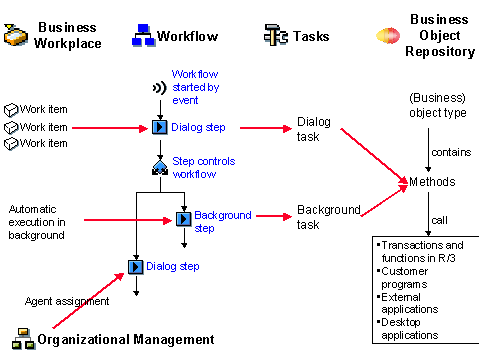
\includegraphics[height=8cm]{Bilder/Business-Workflows_Schema.png}
    \caption[Aufbau eines Business Workflows]{Aufbau eines Business Workflows, Abgerufen von \cite{sap_business-workflows_2022-1} am 17.07.2023.}
    \label{fig:iso_norm}
\end{figure}

Der Business Workplace ist der Ort in einem SAP-System, in dem der Endanwender ''work items'' (übersetzt aus dem Englischen: ''Arbeitspakete'' oder ''Aufgaben'') abhängig vom Zeitpunkt im Geschäftsprozess und den Berechtigungen des Users ausführen kann. Ein work item stellt zur Laufzeit des BW einen Schritt des Prozesses dar, der ausgeführt wird. Es werden hier jedoch nicht alle work items angezeigt. So werden \zB solche, die einem Prozess-Schritt, der im Hintergrund ausgeführt werden soll, zugeordnet sind, hier nicht angezeigt. \footcite[Vgl.][]{sap_business-workflows_2022-1}

Ein Workflow muss vor Ausführung in der ''workflow definition'' angelegt werden. Diese Definition legt die Reihenfolge der auszuführenden Schritte des Prozesses fest und enthält zudem Kontrollschritte. Zusätzlich können noch Bearbeiter und Fristen für bestimmte Schritte festgelegt werden, die dann zur Laufzeit des Workflows vom ''Work item manager'' verwaltet werden. Es gibt viele Arten von Schritten, die gängigen Konzepten in der Programmierung ähneln, wie \zB normale Aktivitäten, Fallunterscheidungen, Schleifen. Zudem gibt es Schritte zum Versenden von Nachrichten, Auslösen von Events, Benutzerentscheidungen, usw. Diese Schritte können entweder im Dialog mit einem Benutzer ausgeführt werden, wenn \zB die Eingabe bestimmter Werte erforderlich ist, oder automatisch vom System im Hintergrund ausgeführt werden. Ein Workflow kann nicht nur manuell von einem Benutzer gestartet werden, sondern auch systemseitig von einem bestimmten Event ausgelöst werden. Hierfür muss in der Definition des Workflows das gewünschte Event als Auslöser angegeben werden. Wenn dann das Event auftritt, wird der Workflow automatisch gestartet. Im betrieblichen Kontext könnte hier \zB ein Mitarbeiter einen Urlaubsantrag stellen, der dann den als Workflow abgebildeten Genehmigungsprozess auslöst. Das wäre ein Beispiel für einen asynchronen Prozess mit sequentieller Kommunikation. \footcite[Vgl.][]{sap_business-workflows_2022-1}

Die einzelnen Schritte, die innerhalb des Workflows ausgeführt werden, hei{\ss}en Tasks und stellen grundlegende betriebliche Tätigkeiten dar. Die Dialog- und Hintergrund-Schritte in der Workflow Definition korrespondieren hier mit Dialog- oder Hintergrund-Tasks. Im Workflow bezieht sich ein Task immer auf eine Methode eines Objekttyps. Diese Methoden können automatisch ausführbar sein oder müssen aktiv von einem Benutzer gestartet werden. Eine Methode kann einerseits Transaktionen oder Funktionen innerhalb des ERP-Systems aufrufen. Spezielle Anforderungen können durch kundeneigene Logik, oder Schnittstellen zu anderen Systemen umgesetzt werden. \footcite[Vgl.][]{sap_business-workflows_2022-1}

Methoden, die innerhalb eines Workflows aufgerufen werden, sind immer Teil von Objekten. Diese Objekte können auch BOs sein. Im Allgemeinen ist ein Objekt ein konkreter Datensatz eines Objekttyps. Die Daten des Objekts werden durch seine Attribute definiert und die Aktionen, wie das Erstellen, Aktualisieren oder Löschen von Daten wird durch die Methoden des Objekts beschrieben. Einen weiteren wichtigen Teil von Objekten stellen Events dar. Diese werden ausgelöst, wenn bei einem Objekt seinen Status verändert. Das kann \zB durch das Erstellen, Verändern oder Löschen von Daten passieren. Diese Events können dann unter anderem Workflows starten. Das ''Business Object Repository'' bietet eine Übersicht über alle in einem SAP-System verfügbaren Objekttypen. Man kann die bereits vorhandenen Objekttypen bei Bedarf anpassen oder neue erstellen. \footcite[Vgl.][]{sap_business-workflows_2022-1}

\subsection{Business Events}

Der zweite Ansatz ist die Umsetzung mit Business Events (BE abgekürzt). Business Events sind Events die von BOs erzeugt und konsumiert werden können. Dieser eventgesteuerte Kommunikationsansatz, der die asynchrone Kommunikation zwischen dem Event-erzeugenden und -konsumierenden BO ermöglicht, wird von RAP im Standard unterstützt. Hier ist keine direkte Antwort des Empfängers nötig, ein BO erzeugt ein Event und dieses wird von anderen BOs dann weiterverarbeitet, ohne dass der Erzeuger weiterhin in diesen Prozess involviert ist Somit spricht man hier von einer einseitigen, also asynchronen Kommunikation. 
Ein BE stellt eine signifikante Veränderung eines BO dar, die im Zuge eines Behaviours erzeugt wird. Dem Event werden dann über dessen Metadaten alle nötigen Informationen, anhand derer die Weiterverarbeitung, je nach speziellem Anwendungsfall, stattfindet, mitgegeben. \footcite[Vgl.][]{sap_business-events_2023}

Ein BO kann als Event-Erzeuger oder Event-Konsument auftreten. Zuerst wird die Erzeuger-Seite betrachtet.

\begin{figure}[H]
    \centering
    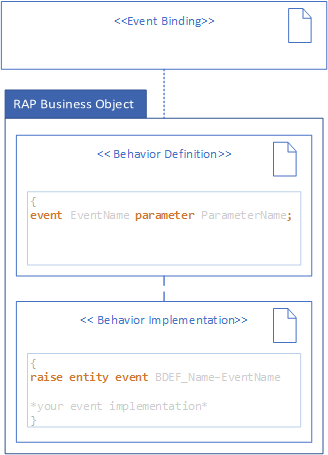
\includegraphics[height=8cm]{Bilder/Business-Events_BO-as-event-consumer.png}
    \caption[Business Object als Event-Erzeuger]{Business Object als Event-Erzeuger, Abgerufen von \cite{sap_business-events_2023} am 17.07.2023.}
    \label{fig:iso_norm}
\end{figure}

Ein Event wird in der Behaviour Definition eines BO erstmals definiert. Hier können dann Parameter für die weitere Verarbeitung mitgegeben werden, die dann in den Metadaten des Events mitgeschickt werden. Danach kann es in der dazugehörigen Behaviour Implementation innerhalb einer spziellen Operation des BO erzeugt werden. Ein Event wird zu dem Zeitpunkt in RAP Laufzeit erzeugt, nachdem die Veränderungen des BO, die das Event auslösen, auf der Datenbank persistiert wurden. Durch das Event Binding wird das Event noch einem speziellen Namensraum, BO und zugehöriger Operation zugeordnet. \footcite[Vgl.][]{sap_business-events_2023}

BOs können BEs nicht nur erzeugen, sonder nauch verarbeiten. Dies geschieht über das Event Consumption Model. Ein Event Consumption Model besteht aus einer Reihe von ABAP-Artefakten, mit denen man Events im SAP-System konsumieren kann. Diese Events müssen jedoch dem Standard eines Cloud Events entsprechen, da der Austausch über das SAP Event Mesh abgewickelt wird, was ein Dienst der SAP Business Technology Platform und somit komplett cloud-basiert ist. Hierfür muss ein inbound bzw. outbound Event-Binding für ein- bzw. ausgehende Events erstellt werden. Diese Bindings sind Teil des SAP Enterprise Event Enablement Frameworks, das den Austausch von Events zwischen dem S/4 System und der BTP regelt. \footcite[Vgl.][]{sap_creating_2022}

\subsection{Background Processing Framework}

Die letzte Möglichkeit, die betrachtet wird, um asynchrone Prozesse abzubilden, stellt das ''background Processing Framework'' (bgPF abgekürzt) dar.

Das bgPF ist ein Framework, das die Möglichkeit schafft asynchron zum Hauptprozess Logik auszulagern und auszuführen. Zuerst soll auf die grundlegende Funktionsweise des bgPF eingegangen werden.

\begin{figure}[H]
    \centering
    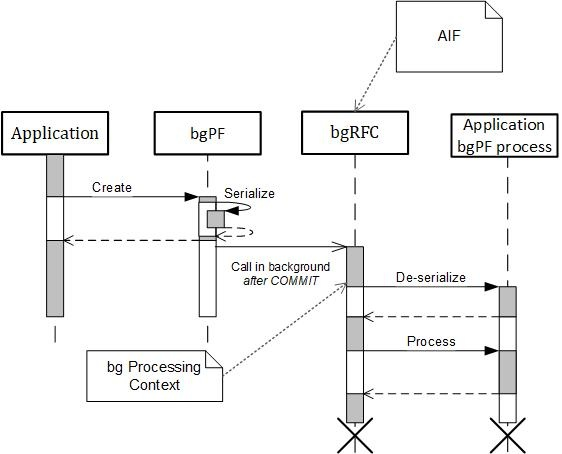
\includegraphics[height=8cm]{Bilder/bgPF_Schema.png}
    \caption[Funktionsweise des bgPF]{Funktionsweise des bgPF, Abgerufen von \cite{sap_bgpf_2023} am 17.07.2023.}
    \label{fig:iso_norm}
\end{figure}

Nachdem das Interface für das bgPF in der Anwendung als eigene Klasse mit der jeweiligen Logik, die ausgelagert werden soll, implementiert wurde, kann es verwendet werden. Die Anwendung ruft dann zur Laufzeit diese Klasse auf und erstellt synchron ein bgPF-Objekt. Innerhalb dieses Objekts wird die Klasse dann serialisiert und mit einem Methodenaufruf für die spätere Ausführung gespeichert. In der Endphase des Hauptprozesses wird dann mit einem bgRFC, also einem Funktionsaufruf, der im Hintergrund ausgeführt wird, die Ausführung ausgelöst. Der bgRFC wird dann in einer neuen ABAP Laufzeit als neuer Prozess gestartet. Hier wird die serialisierte Klasse wieder deserialisiert und die implementierte Logik ausgeführt. Nach dem Ausführen wird der Prozess wieder beendet. Falls nötig, können durch das Bereitstellen eines eigenen Verarbeitungskontexts von der aufrufenden Anwendung spezifische Verarbeitungsprioritäten festgelegt werden. Dies ist zwingend notwendig, wenn die Verarbeitungsreihenfolge genau eingehalten werden muss. Der voreingestellte Kontext wird standardäßig von anderen Anwendungen gemeinsam verwendet. \footcite[Vgl.][]{sap_bgpf_2023}

Das Entkoppeln und asynchrone Ausführen gewisser Logik vom Hauptprozess bringt einige Vorteile mit sich: Zuerst wird die Robustheit und transaktionale Konsistenz des Hauptprozesses und somit auch die Konsistenz der Daten sichergestellt. Das bgPF bietet die Möglichkeit, diese Konsistenz zu gewährleisten, aber auch gleichzeitig relevantes Coding aus dem Hauptprozess auszulagern, was dessen Robustheit verbessert. Des Weiteren erscheint die Hauptanwendung für den Benutzer performanter, da gewisse Verarbeitungslogik in einer anderen Sitzung asynchron ausgeführt werden kann. Ein weiterer Vorteil ist die bessere Skalierbarkeit, wenn grö{\ss}ere Prozesse in kleinere Teile unterteilt werden, die verteilt über mehrere Laufzeitumgebungen asynchron ausgeführt werden können. Die Skalierung einer Anwendung kann mit dieser Technologie dann komplett vom SAP-System automatisiert werden. \footcite[Vgl.][]{sap_bgpf_2023}

\subsubsection{bgPF innerhalb von RAP}

Das bgPF kann auch innerhalb von RAP verwendet werden. Grundlegend besteht die Laufzeit eines RAP BOs aus einer Interaktions- und einer Speicherungsphase. In der Interaktionsphase werden über die Behaviours des BO dessen Daten ausgelesen oder verändert. Falls Änderungen an den Daten stattgefunden haben, werden diese jedoch nicht direkt auf der Datenbank persistiert, sondern zuerst in einem Puffer gespeichert. Nachdem alle Änderungen erfolgreich durchgeführt wurden, werden diese auf einmal in der Speicherungsphase auf die Datenbank geschrieben. Konkret wird die Methode des bgPF-Objekts, die das Speichern für die spätere asynchrone Ausführung übernimmt, in der zweiten Phase der Laufzeit des BOs aufgerufen und das Objekt somit auf der Datenbank gespeichert. \footcite[Vgl.][]{sap_bgpf_2023}

\section{Vergleich der Ansätze}

Im Folgenden sollen die in den vorherigen Kapiteln vorgestellten Ansätze miteinander verglichen werden. Hierfür werden die Kriterien Komplexität der Implementierung, also welchen Aufwand das Umsetzen der Technologie im Anwendungsfall verursacht, die Auswirkungen auf die Systemlandschaft, also ob zusätzliche Systemkomponenten benötigt werden und die Performance der einzelnen Ansätze im Bezug auf Ausführungsdauer und Rechenlast verglichen werden. Weitere Kriterien sind zusätzliche Kosten die eine Lösung eventuell verursacht, die Abwärtskompatibilität zu älteren Systemen und die Flexibilität der Technologien im Bezug auf Gestaltungsmöglichkeiten von Anwendungsszenarien und Integration mit anderen Technologien/ Frameworks. Abgeschlossen wird der Vergleich mit einer Betrachtung der Skalierbarkeit und Wartbarkeit der drei Umsetzungsmöglichkeiten.

\subsubsection{Komplexität der Implementierung}



\subsubsection{Auswirkungen auf die Systemlandschaft}



\subsubsection{Performance}



\subsubsection{Kosten}



\subsubsection{Flexibilität}



\subsubsection{Skalierbarkeit}



\subsubsection{Wartbarkeit}



\section{Entscheidungsmatrix}

Hier soll eine Entscheidungsmatrix entwickelt werden, welchen Lösungsansatz man in Abhängigkeit von mehreren Faktoren am besten verwenden soll (ersetzt auch weng mit die Zusammenfassung)
\newline

Experteninterviews:

- BusinessEvents (Martin Müller (+bgpf), Marcel Herrmanns, Daniel Wachs) \newline
- Business Workflows (Eric Gheris) \newline
- bgPF ?

mögliche Vergleichskriterien:

- Komplexität der Implementierung (Ranking: Workflow > Business Events > bgPF) -> Lines of Code, Artefakte \newline
- Systemlandschaft (Cloudkomponente (Datenschutz) EventMesh von BTP bei Business Events nötig, bgPF/ Workflows brauchen das nicht) \newline
- Performance (Rechenlast, Zeit) (BE nicht so gut, weil Kommunikation über Web zu Cloud über HTTP, bgPF <-> Workflows nehmen sich nicht viel) \newline
- Kosten (Vorteil Workflows: Release (Abwärts-) Kompatibilität zu ECC (gibts schon immer), Drängen von Kunden auf Funktionsverfügbarkeit in alten Systemen) (BE: Lizenzkosten für BTP Komponente, Netzwerklast durch HTTP Kommunikation bei Kunde) \newline
- Flexibilität (Workflows sehr flexibel, viele Anbindungen, sehr gute Integration zu zB. Emails) (Beiden anderen Techniken eher low level Code, wenig Anbindungen an andere Frameworks) \newline
- Skalierbarkeit (Workflows (nicht aufteilbar), BE überhaupt nicht) (bgPF Autoskalierbar, -> siehe Praxiskapitel) \newline
- Wartbarkeit (Workflows extrem gut wartbar -> komplett auf ABAP-Instanz debuggbar/ nachvollziehbar) (bgPF ähnlich) (BE schlechte Wartbarkeit, da über viele Systeme, Frameworks, intransparente Analysemöglichkeiten)